\begin{mainquestion}{zenerregulator}{Solar Panel Zener Diode}

You are working at a company that builds solar chargers for campers. You have been tasked with regulating the output of a solar panel to \qty{12}{\volt} - \qty{14}{\volt}. The source voltage $V_{DC}$ models the solar panel and is known to vary between \qty{13.7}{\volt} and \qty{23.4}{\volt} depending on the cloud cover. For the target application, you should expect to see anywhere between 0 and \qty{100}{\milli\ampere} of load current, depending on conditions. You remember from EE101A that zener diodes can regulate voltage, so you start your design with the below circuit.

\begin{center}
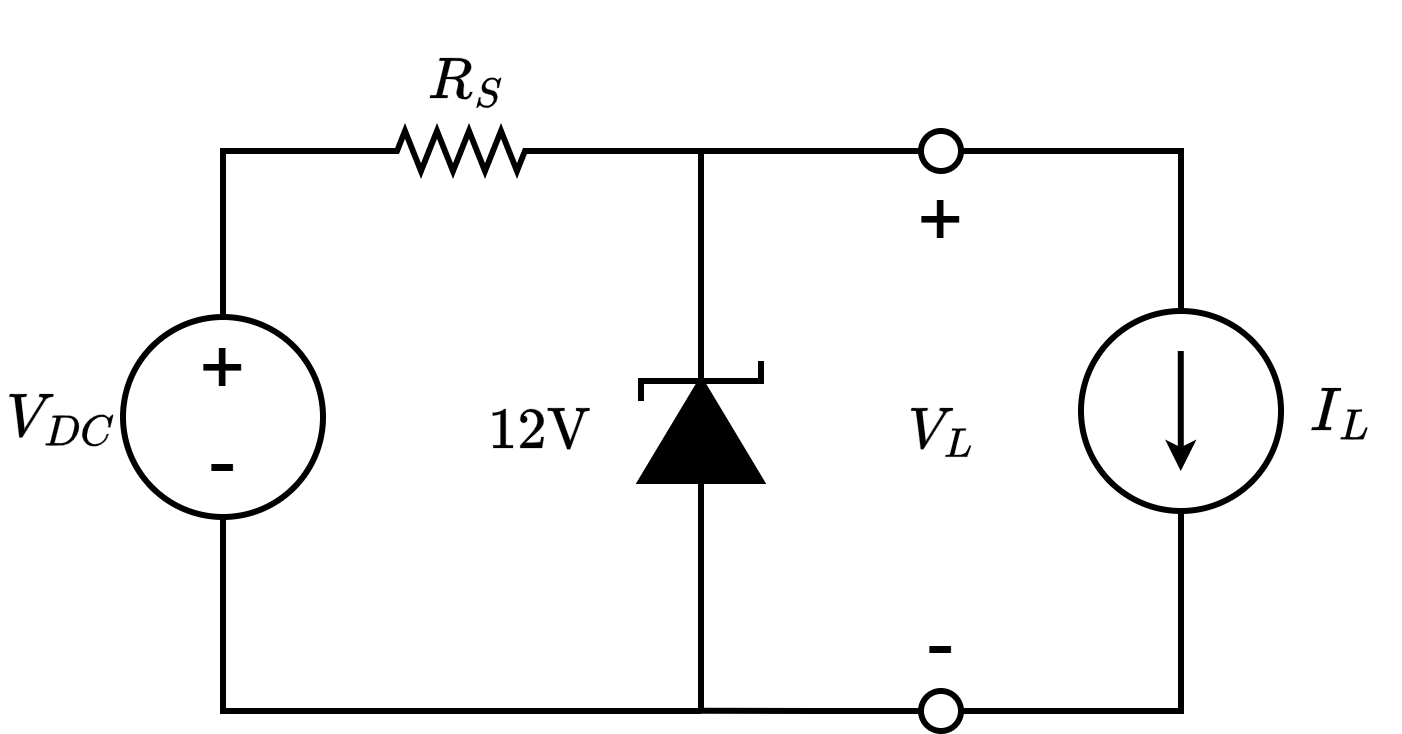
\includegraphics[width=3.5in]{questionbank/diodes/zener_regulator/v1/zener_circuit.png}
\end{center}

% =========================================================
\begin{partquestion}{inadequatedesign}
{Initially you are told that the source resistance of the panel is $R_S = \qty{50}{\ohm}$. Show it is not possible to maintain $V_L$ across the desired range of parameters.}

\begin{answer}
The zener diode can maintain the desired voltage as long as we keep it in breakdown mode. This is possible unless the voltage drop across the resistor is such that the zener diode voltage drops under its rated breakdown value. In equation form:

\[
V_L = V_{DC} - (I_D + I_L) R_S
\]

This is lowest when $V_{DC}$ is at its minimum value, and when $I_L$ is at its maximum value. Plugging in these given values leads to:

\begin{align*}
V_L &= 13.7 - (I_D + 0.1) 50 \\
&= 8.7 - 50I_D
\end{align*}

which will be much less than the desired voltage level at 12 V. (Note that $I_D$ is non-negative; it is zero when the diode is not conducting and some positive value when it is operating in breakdown mode.) Clearly this value of resistor is too large!
\end{answer}
\end{partquestion}

% =========================================================
\begin{partquestion}{maxresistor}
{What is the maximum value of $R_S$ that prevents $V_L$ from dropping below the desired range if the zener diode breakdown voltage is $V_{Z0} = 12\text{ V}$?}

\begin{answer}
We can reuse the formula from the previous part:

\[
V_L = V_{DC} - (I_D + I_L) R_S
\]

and consider the case where we are in breakdown, such that $V_L \geq V_{Z0} = 12\text{ V}$. We have:

\begin{align*}
V_{DC,\text{min}} - (I_D + I_L) R_S &\geq V_{Z0} \\
V_{DC,\text{min}} - I_L R_S &\geq V_{Z0} \\
R_S &\leq \frac{V_{DC,\text{min}} - V_{Z0}}{I_L} = \frac{13.7 - 12}{0.1} \\
R_S &\leq \qty{17}{\ohm}
\end{align*}
Equality is theoretically reached at the very edge of zener breakdown, but practically, the diode no longer maintains a meaningful breakdown current and a regulator would likely require a smaller resistance.
\end{answer}
\end{partquestion}

% =========================================================
\begin{partquestion}{zenercurrent}
{With your updated $R_S$, what is $I_D$ when $V_{DC}$ is at a maximum and the current load $I_L$ is zero? What is the power dissipated in the diode in this case?}

\begin{answer}
When the current load is zero, the load is an open circuit and all the current will flow through the zener diode. We can calculate:

\begin{align*}
I_D &= \frac{V_{DC,\text{max}} - V_{Z0}}{R_S} \\
&= \frac{23.4 - 12}{17} \approx \qty{671}{\milli\ampere}
\end{align*}

The power is easy to find now that we have the voltage and current:
\[P_D = V_D \cdot I_D = 12 \cdot 0.67 = \qty{8.05}{\watt}\]

\end{answer}
\end{partquestion}

\begin{partquestion}{search}
{Search \href{https://www.digikey.com/}{Digikey} and \href{https://www.mouser.com/?srsltid=AfmBOoo5j27SqCXjzHUROxjIwUmXG71N7j6Ma3DKRVKD3fQJOXdC2enf}{Mouser} for a zener diode that will fit your specifications. How much does it cost? Could you build this circuit for less than \$10?}

\begin{answer}
The \href{https://www.mouser.com/datasheet/3/282/1/1N2970B-3015B.1N3993A-3998A.pdf}{1N2976B} is a 12V Zener diode that can handle 10W, but it cost over \$30! It's unlikely you could get this built for less than \$10 unless you get some bulk discounts. Real regulators use a different circuit called a buck converter to reduce the voltage. Take Power Electronics (EE153) to learn how to regulate large voltages and currents.
\end{answer}
\end{partquestion}


\end{mainquestion}
